% Verification of the vector-addition and dot-product programs on the Kites RISC-V simulator,
% with the scalar vs. vector comparison.
%
% Build:  pdflatex verification.tex   (run twice for the references)
% The tables in tables/ and the figure speedup_vs_n.pdf are generated from the simulator runs by
%   python benchmarks/edge_cases.py
% so every number in them is a measured value.
\documentclass[11pt,a4paper]{article}

\usepackage[margin=2.2cm]{geometry}
\usepackage[T1]{fontenc}
\usepackage{lmodern}
\usepackage{amsmath,amssymb}
\usepackage{booktabs}
\usepackage{array}
\usepackage{graphicx}
\usepackage{xcolor}
\usepackage{listings}
\usepackage{pifont}
\usepackage{caption}
\usepackage{float}
\usepackage[hidelinks]{hyperref}

\newcommand{\cmark}{\textcolor{green!45!black}{\ding{51}}}
\newcommand{\xmark}{\textcolor{red!70!black}{\ding{55}}}
\newcommand{\code}[1]{\texttt{#1}}
% generated by benchmarks/edge_cases.py -- do not edit
\newcommand{\runsTotal}{118}
\newcommand{\runsPassed}{118}


\definecolor{cmt}{RGB}{110,110,104}
\definecolor{kw}{RGB}{30,90,170}
\lstdefinestyle{asm}{
  basicstyle=\ttfamily\footnotesize,
  commentstyle=\color{cmt}\itshape,
  morecomment=[l]{\#},
  alsoletter={.},
  keywordstyle=\color{kw}\bfseries,
  morekeywords={vsetvli,vle32.v,vse32.v,vadd.vv,vmul.vv,vredsum.vs,vmv.s.x,vmv.x.s},
  columns=fullflexible,
  keepspaces=true,
  frame=single,
  rulecolor=\color{black!25},
  xleftmargin=1.2em,
  framexleftmargin=1em,
  aboveskip=6pt,
  belowskip=6pt
}
\captionsetup{font=small,labelfont=bf}

\title{Vector addition and dot product on the Kites simulator:\\
       verification, edge cases and scalar vs.\ vector statistics}
\author{RISC-V Vector Extension (RVV 1.0) project}
\date{\today}

\begin{document}
\maketitle

\begin{abstract}
Two common vector kernels, element-wise \emph{vector addition} ($c_i = a_i + b_i$) and the
\emph{dot product} ($\sum_i a_i b_i$), were written in RISC-V assembly twice: once with the
base integer instructions only (RV64IM, ``scalar'') and once with the vector extension
(RVV~1.0, ``vector''). This document describes how both versions were checked on the Kites
simulator, including edge cases (array lengths around the vector length, a single element, an
empty array, very long arrays, 32-bit overflow, several vector register lengths and the pipelined
processors), and compares the two versions using the statistics collected by the simulator.
All \runsPassed{} of \runsTotal{} test runs produced exactly the expected result, and on the
single-cycle VM every measured instruction count equalled the predicted one. For long arrays the vector versions execute about
\textbf{26$\times$} (addition) and \textbf{25$\times$} (dot product) fewer instructions at
VLEN~=~128~bits, and over 150$\times$ fewer at VLEN~=~1024~bits.
\end{abstract}

\tableofcontents

%==============================================================================================
\section{The programs}
%==============================================================================================

Both kernels work on 32-bit signed integers (\code{int32\_t}). The inputs \code{a} and
\code{b} are in the program's \code{.data} section; the result is written to the label
\code{out} at address \code{0x10000000}. The full, commented programs are in
\code{benchmarks/programs/} (\code{vadd\_scalar.s}, \code{vadd\_vector.s}, \code{dot\_scalar.s},
\code{dot\_vector.s}). Only the code sections are shown here. The element count $N$ is the
operand of \code{li a3, N}.

\subsection{Vector addition}

\begin{minipage}[t]{0.47\textwidth}
\textbf{Scalar} (one element per iteration)
\begin{lstlisting}[style=asm]
    la   a0, a        # &a[0]
    la   a1, b        # &b[0]
    la   a2, out      # &c[0]
    li   a3, N        # elements left
loop:
    lw   t0, 0(a0)    # a[i]
    lw   t1, 0(a1)    # b[i]
    add  t0, t0, t1   # a[i] + b[i]
    sw   t0, 0(a2)    # c[i]
    addi a0, a0, 4
    addi a1, a1, 4
    addi a2, a2, 4
    addi a3, a3, -1
    bnez a3, loop
\end{lstlisting}
\end{minipage}\hfill
\begin{minipage}[t]{0.50\textwidth}
\textbf{Vector} (up to VLMAX elements per pass)
\begin{lstlisting}[style=asm]
    la   a0, a
    la   a1, b
    la   a2, out
    li   a3, N
loop:
    vsetvli t0, a3, e32, m8, ta, ma # vl
    vle32.v v0, (a0)      # a[i..i+vl-1]
    vle32.v v8, (a1)      # b[i..i+vl-1]
    vadd.vv v16, v0, v8   # vl sums
    vse32.v v16, (a2)     # c[i..i+vl-1]
    slli t1, t0, 2        # vl * 4 bytes
    add  a0, a0, t1
    add  a1, a1, t1
    add  a2, a2, t1
    sub  a3, a3, t0       # vl done
    bnez a3, loop
\end{lstlisting}
\end{minipage}

\subsection{Dot product}

\begin{minipage}[t]{0.47\textwidth}
\textbf{Scalar}
\begin{lstlisting}[style=asm]
    la   a0, a
    la   a1, b
    la   a2, out
    li   a3, N
    li   a4, 0        # sum
loop:
    lw   t0, 0(a0)
    lw   t1, 0(a1)
    mul  t0, t0, t1   # a[i] * b[i]
    add  a4, a4, t0   # sum += ...
    addi a0, a0, 4
    addi a1, a1, 4
    addi a3, a3, -1
    bnez a3, loop
    sw   a4, 0(a2)    # out = sum
\end{lstlisting}
\end{minipage}\hfill
\begin{minipage}[t]{0.50\textwidth}
\textbf{Vector}
\begin{lstlisting}[style=asm]
    la   a0, a
    la   a1, b
    la   a2, out
    li   a3, N
    vsetvli t0, x0, e32, m1, ta, ma
    vmv.s.x v24, zero     # v24[0] = 0
loop:
    vsetvli t0, a3, e32, m8, ta, ma
    vle32.v v0, (a0)
    vle32.v v8, (a1)
    vmul.vv v16, v0, v8   # vl products
    vredsum.vs v24, v16, v24 # v24[0] += sum
    slli t1, t0, 2
    add  a0, a0, t1
    add  a1, a1, t1
    sub  a3, a3, t0
    bnez a3, loop
    vmv.x.s a4, v24       # a4 = v24[0]
    sw   a4, 0(a2)
\end{lstlisting}
\end{minipage}

\subsection{Strip-mining and VLMAX}

The vector loops are \emph{strip-mined}: in every pass \code{vsetvli} sets
\[
  vl = \min(\text{elements left},\ \mathrm{VLMAX}), \qquad
  \mathrm{VLMAX} = \frac{\mathrm{LMUL}\cdot\mathrm{VLEN}}{\mathrm{SEW}}
               = \frac{8\cdot\mathrm{VLEN}}{32} = \frac{\mathrm{VLEN}}{4},
\]
so with the default VLEN~=~128~bits one vector instruction processes up to 32 elements. The
number of passes and the length of the last pass are
\[
  P(N) = \left\lceil \frac{N}{\mathrm{VLMAX}} \right\rceil, \qquad
  vl_{\text{last}} = N - (P-1)\cdot\mathrm{VLMAX}.
\]
The same binary therefore works for every $N$ and every VLEN; nothing in the code depends on
either.

%==============================================================================================
\section{How the programs were checked}
%==============================================================================================

\subsection{Test procedure}

The checks are automated by \code{benchmarks/edge\_cases.py} (the five standard benchmarks by
\code{benchmarks/run\_benchmarks.py}). For every test case:

\begin{enumerate}
  \item \textbf{Generate the program.} The code section of the original program is used
        unchanged. Only the operand of \code{li a3, N} and the \code{.data} section (the arrays
        \code{a}, \code{b} and the output area) are replaced. The output area is followed by a
        64-byte \emph{guard area} filled with zeros.
  \item \textbf{Run it on Kites} with the command-line front end, which assembles the file,
        loads it, runs it to the end and dumps the requested memory:
\begin{lstlisting}[style=asm,frame=none,xleftmargin=0pt]
kites-cli prog.s --vm rvss --vlen 128 --stats --mem-dump 0x10000000 <rows>
\end{lstlisting}
        \code{--stats} makes the simulator classify every executed instruction (single-cycle
        VM) and write \code{vm\_state/stats\_dump.json}.
  \item \textbf{Compute the expected result in Python} from the same input arrays (the
        reference model, Section~\ref{sec:ref}).
  \item \textbf{Compare.} A case passes only if \emph{all} of these hold:
  \begin{itemize}
    \item the program exits normally and the simulator reports no error;
    \item the bytes at \code{out} are exactly the expected 32-bit results;
    \item the guard area after \code{out} is still all zero, i.e.\ no store went past the last
          element (important for the last, partial vector pass);
    \item on the single-cycle VM, the dynamic instruction count equals the analytic count of
          Section~\ref{sec:model};
    \item for the vector programs, the total number of vector elements processed (sum of
          $vl$ over all vector instructions, from the simulator's statistics) equals the
          expected work: $4N$ for addition (two loads, one add, one store per element) and
          $4N+2$ for the dot product (two loads, one multiply and one reduction per element,
          plus \code{vmv.s.x} and \code{vmv.x.s} which each touch one element).
  \end{itemize}
\end{enumerate}

\subsection{Reference model and 32-bit overflow}\label{sec:ref}

The reference uses 32-bit two's-complement wrap-around, written $\mathrm{wrap}(x)$:
\[
  c_i = \mathrm{wrap}(a_i + b_i), \qquad
  \text{dot} = \mathrm{wrap}\!\Big(\sum_{i=0}^{N-1} a_i\, b_i\Big), \qquad
  \mathrm{wrap}(x) = \big((x + 2^{31}) \bmod 2^{32}\big) - 2^{31}.
\]
The scalar and vector dot products compute this in different ways. The scalar program runs on
RV64: \code{lw} sign-extends to 64 bits, \code{mul} and \code{add} work on 64 bits and only the
final \code{sw} keeps the low 32 bits. The vector program uses SEW~=~32: \code{vmul.vv} keeps
the low 32 bits of each product and \code{vredsum.vs} adds modulo $2^{32}$. Because addition and
multiplication are compatible with reduction modulo $2^{32}$, both give
$\big(\sum a_i b_i\big) \bmod 2^{32}$, so both must match the reference bit for bit even when
the intermediate values overflow. The ``extremes'' and ``full range'' test patterns check
exactly this.

\subsection{Checking the checker}

Two deliberately wrong programs were run through the same procedure to make sure a wrong result
cannot pass:
\begin{itemize}
  \item \textbf{Store past the end:} a program that processes 32 elements while the expected
        result and output area are for 31. The first 31 results are correct, but the guard check
        fails for both the scalar and the vector version.
  \item \textbf{Wrong data:} one input value in the program differs by 1 from the reference
        input. The result check fails for all four programs.
\end{itemize}
Both were reported as failures, as they should be.

%==============================================================================================
\section{Edge cases and results}
%==============================================================================================

\subsection{Array length}

The lengths were chosen around the points where the vector loop changes behaviour:
\begin{itemize}
  \item $N=1, 2, 7$: fewer elements than VLMAX; one partial pass.
  \item $N=31, 32, 33$: just below, exactly at, and just above VLMAX~=~32. $N=33$ needs a
        second pass with $vl=1$.
  \item $N=64$ and $N=100$: two full passes; three full passes plus a tail of 4.
  \item $N=255, 256, 257$: around the size of the standard benchmark.
  \item $N=1000$ and $N=4096$: long arrays (tail of 8, and 128 full passes).
  \item $N=0$: empty array, vector version only. \code{vsetvli} returns $vl=0$, so the loads,
        the arithmetic and the reduction do nothing (for $vl=0$ the RVV specification
        leaves the destination unchanged), the counter stays 0 and the loop exits after one
        pass. The dot product correctly stores 0. The hand-written scalar loops are
        \emph{do--while} loops and require $N \ge 1$ (with $N=0$ the counter would wrap
        to $2^{64}-1$), like compiled code after the compiler has checked $N > 0$, so $N=0$
        was not run for them.
\end{itemize}

Tables~\ref{tab:len-vadd} and~\ref{tab:len-dot} list every run at VLEN~=~128. The instruction
counts are measured; the value in brackets is the count predicted by the model of
Section~\ref{sec:model}. All of them agree exactly.

\begin{table}[H]
\centering\small
\caption{Vector addition, VLEN~=~128 (VLMAX~=~32). IC = dynamic instruction count, measured
(model). Elements = sum of $vl$ over all vector instructions.}
\label{tab:len-vadd}
\begin{tabular}{rrrrrrrc}
\toprule
$N$ & passes & last $vl$ & IC scalar & IC vector & speedup & elements & passed \\
\midrule
% generated by benchmarks/edge_cases.py -- do not edit
0 & 1 & 0 & \emph{not run} & 18 (18) & -- & 0 & \cmark \\
1 & 1 & 1 & 16 (16) & 18 (18) & 0.89 & 4 & \cmark \\
2 & 1 & 2 & 25 (25) & 18 (18) & 1.39 & 8 & \cmark \\
7 & 1 & 7 & 70 (70) & 18 (18) & 3.89 & 28 & \cmark \\
31 & 1 & 31 & 286 (286) & 18 (18) & 15.89 & 124 & \cmark \\
32 & 1 & 32 & 295 (295) & 18 (18) & 16.39 & 128 & \cmark \\
33 & 2 & 1 & 304 (304) & 29 (29) & 10.48 & 132 & \cmark \\
64 & 2 & 32 & 583 (583) & 29 (29) & 20.10 & 256 & \cmark \\
100 & 4 & 4 & 907 (907) & 51 (51) & 17.78 & 400 & \cmark \\
255 & 8 & 31 & 2{,}302 (2{,}302) & 95 (95) & 24.23 & 1{,}020 & \cmark \\
256 & 8 & 32 & 2{,}311 (2{,}311) & 95 (95) & 24.33 & 1{,}024 & \cmark \\
257 & 9 & 1 & 2{,}320 (2{,}320) & 106 (106) & 21.89 & 1{,}028 & \cmark \\
1{,}000 & 32 & 8 & 9{,}007 (9{,}007) & 359 (359) & 25.09 & 4{,}000 & \cmark \\
4{,}096 & 128 & 32 & 36{,}871 (36{,}871) & 1{,}415 (1{,}415) & 26.06 & 16{,}384 & \cmark \\

\bottomrule
\end{tabular}
\end{table}

\begin{table}[H]
\centering\small
\caption{Dot product, VLEN~=~128 (VLMAX~=~32).}
\label{tab:len-dot}
\begin{tabular}{rrrrrrrc}
\toprule
$N$ & passes & last $vl$ & IC scalar & IC vector & speedup & elements & passed \\
\midrule
% generated by benchmarks/edge_cases.py -- do not edit
0 & 1 & 0 & \emph{not run} & 21 (21) & -- & 2 & \cmark \\
1 & 1 & 1 & 17 (17) & 21 (21) & 0.81 & 6 & \cmark \\
2 & 1 & 2 & 25 (25) & 21 (21) & 1.19 & 10 & \cmark \\
7 & 1 & 7 & 65 (65) & 21 (21) & 3.10 & 30 & \cmark \\
31 & 1 & 31 & 257 (257) & 21 (21) & 12.24 & 126 & \cmark \\
32 & 1 & 32 & 265 (265) & 21 (21) & 12.62 & 130 & \cmark \\
33 & 2 & 1 & 273 (273) & 31 (31) & 8.81 & 134 & \cmark \\
64 & 2 & 32 & 521 (521) & 31 (31) & 16.81 & 258 & \cmark \\
100 & 4 & 4 & 809 (809) & 51 (51) & 15.86 & 402 & \cmark \\
255 & 8 & 31 & 2{,}049 (2{,}049) & 91 (91) & 22.52 & 1{,}022 & \cmark \\
256 & 8 & 32 & 2{,}057 (2{,}057) & 91 (91) & 22.60 & 1{,}026 & \cmark \\
257 & 9 & 1 & 2{,}065 (2{,}065) & 101 (101) & 20.45 & 1{,}030 & \cmark \\
1{,}000 & 32 & 8 & 8{,}009 (8{,}009) & 331 (331) & 24.20 & 4{,}002 & \cmark \\
4{,}096 & 128 & 32 & 32{,}777 (32{,}777) & 1{,}291 (1{,}291) & 25.39 & 16{,}386 & \cmark \\

\bottomrule
\end{tabular}
\end{table}

\subsection{Data values}

Table~\ref{tab:patterns} shows the data patterns. The inputs of the length tests are random
(within $\pm 10^5$ for addition and $\pm 100$ for the dot product). These patterns add the
boundary values. $N=37$ for the ``extremes'' pattern also gives a partial last pass ($vl=5$).

\begin{table}[H]
\centering\small
\caption{Data-pattern edge cases (VLEN~=~128).}
\label{tab:patterns}
\begin{tabular}{llr>{\raggedright\arraybackslash}p{6.4cm}cc}
\toprule
Kernel & pattern & $N$ & what it tests & scalar & vector \\
\midrule
% generated by benchmarks/edge_cases.py -- do not edit
Vector addition & zeros & 256 & all inputs 0 & \cmark & \cmark \\
Vector addition & minus\_one & 256 & all inputs $-1$ (sign extension) & \cmark & \cmark \\
Vector addition & extremes & 37 & operands INT32\_MAX, INT32\_MIN, $-1$, 0: most results overflow 32 bits & \cmark & \cmark \\
Vector addition & full\_range & 256 & random values over the whole int32 range & \cmark & \cmark \\
Dot product & zeros & 256 & all inputs 0 & \cmark & \cmark \\
Dot product & minus\_one & 256 & all inputs $-1$ (sign extension) & \cmark & \cmark \\
Dot product & extremes & 37 & operands INT32\_MAX, INT32\_MIN, $-1$, 0: most results overflow 32 bits & \cmark & \cmark \\
Dot product & full\_range & 256 & random values over the whole int32 range & \cmark & \cmark \\

\bottomrule
\end{tabular}
\end{table}

\subsection{Vector register length (VLEN)}

The vector programs were also run with \code{--vlen 256, 512, 1024} without any change to the
code (Table~\ref{tab:vlen}). The scalar programs do not use vector registers, and their count
was confirmed to be the same at VLEN~=~1024 as at 128.

\begin{table}[H]
\centering\footnotesize\setlength{\tabcolsep}{4.5pt}
\caption{Scaling with VLEN. VLMAX~=~VLEN/4 for e32, m8. The speedup is against the scalar
version with the same $N$.}
\label{tab:vlen}
\begin{tabular}{lrrrrrrrc}
\toprule
Kernel & $N$ & VLEN & VLMAX & passes & IC vector (model) & IC scalar & speedup & passed \\
\midrule
% generated by benchmarks/edge_cases.py -- do not edit
Vector addition & 33 & 128 & 32 & 2 & 29 (29) & 304 & 10.5 & \cmark \\
Vector addition & 33 & 256 & 64 & 1 & 18 (18) & 304 & 16.9 & \cmark \\
Vector addition & 33 & 512 & 128 & 1 & 18 (18) & 304 & 16.9 & \cmark \\
Vector addition & 33 & 1024 & 256 & 1 & 18 (18) & 304 & 16.9 & \cmark \\
\addlinespace[2pt]
Vector addition & 256 & 128 & 32 & 8 & 95 (95) & 2{,}311 & 24.3 & \cmark \\
Vector addition & 256 & 256 & 64 & 4 & 51 (51) & 2{,}311 & 45.3 & \cmark \\
Vector addition & 256 & 512 & 128 & 2 & 29 (29) & 2{,}311 & 79.7 & \cmark \\
Vector addition & 256 & 1024 & 256 & 1 & 18 (18) & 2{,}311 & 128.4 & \cmark \\
\addlinespace[2pt]
Vector addition & 1{,}000 & 128 & 32 & 32 & 359 (359) & 9{,}007 & 25.1 & \cmark \\
Vector addition & 1{,}000 & 256 & 64 & 16 & 183 (183) & 9{,}007 & 49.2 & \cmark \\
Vector addition & 1{,}000 & 512 & 128 & 8 & 95 (95) & 9{,}007 & 94.8 & \cmark \\
Vector addition & 1{,}000 & 1024 & 256 & 4 & 51 (51) & 9{,}007 & 176.6 & \cmark \\
\addlinespace[2pt]
Dot product & 33 & 128 & 32 & 2 & 31 (31) & 273 & 8.8 & \cmark \\
Dot product & 33 & 256 & 64 & 1 & 21 (21) & 273 & 13.0 & \cmark \\
Dot product & 33 & 512 & 128 & 1 & 21 (21) & 273 & 13.0 & \cmark \\
Dot product & 33 & 1024 & 256 & 1 & 21 (21) & 273 & 13.0 & \cmark \\
\addlinespace[2pt]
Dot product & 256 & 128 & 32 & 8 & 91 (91) & 2{,}057 & 22.6 & \cmark \\
Dot product & 256 & 256 & 64 & 4 & 51 (51) & 2{,}057 & 40.3 & \cmark \\
Dot product & 256 & 512 & 128 & 2 & 31 (31) & 2{,}057 & 66.4 & \cmark \\
Dot product & 256 & 1024 & 256 & 1 & 21 (21) & 2{,}057 & 98.0 & \cmark \\
\addlinespace[2pt]
Dot product & 1{,}000 & 128 & 32 & 32 & 331 (331) & 8{,}009 & 24.2 & \cmark \\
Dot product & 1{,}000 & 256 & 64 & 16 & 171 (171) & 8{,}009 & 46.8 & \cmark \\
Dot product & 1{,}000 & 512 & 128 & 8 & 91 (91) & 8{,}009 & 88.0 & \cmark \\
Dot product & 1{,}000 & 1024 & 256 & 4 & 51 (51) & 8{,}009 & 157.0 & \cmark \\

\bottomrule
\end{tabular}
\end{table}

\subsection{Pipelined processors}

The same programs were run on the five-stage pipelined VMs that detect hazards: \code{rv5-h-nf}
(stalls, no forwarding) and \code{rv5-h-f} (stalls and forwarding). This checks that the
results do not depend on the processor model (Table~\ref{tab:pipe}). The \code{rv5-nh-*} VMs
deliberately do \emph{not} detect data hazards (they demonstrate hazards), so wrong results
there are expected and they were not used.

\begin{table}[H]
\centering\small
\caption{Correctness on the pipelined VMs (s = scalar, v = vector).}
\label{tab:pipe}
\begin{tabular}{llcccccc}
\toprule
& & \multicolumn{2}{c}{$N=1$} & \multicolumn{2}{c}{$N=33$} & \multicolumn{2}{c}{$N=256$} \\
\cmidrule(lr){3-4}\cmidrule(lr){5-6}\cmidrule(lr){7-8}
VM & Kernel & s & v & s & v & s & v \\
\midrule
% generated by benchmarks/edge_cases.py -- do not edit
\texttt{rv5-h-nf} & Vector addition & \cmark & \cmark & \cmark & \cmark & \cmark & \cmark \\
\texttt{rv5-h-nf} & Dot product & \cmark & \cmark & \cmark & \cmark & \cmark & \cmark \\
\texttt{rv5-h-f} & Vector addition & \cmark & \cmark & \cmark & \cmark & \cmark & \cmark \\
\texttt{rv5-h-f} & Dot product & \cmark & \cmark & \cmark & \cmark & \cmark & \cmark \\

\bottomrule
\end{tabular}
\end{table}

%==============================================================================================
\section{Scalar vs.\ vector: comparative calculations}\label{sec:model}
%==============================================================================================

\subsection{Instruction-count model}

Counting the instructions in the listings gives the dynamic instruction count (IC) exactly. Each
\code{la} expands to two instructions (\code{auipc}, \code{addi}). Writing
$P = \max\!\big(1, \lceil N/\mathrm{VLMAX} \rceil\big)$ for the number of vector passes:

\begin{center}
\begin{tabular}{lll}
\toprule
& scalar & vector \\
\midrule
Vector addition &
  $\underbrace{7}_{3\,\texttt{la},\ \texttt{li}} + \underbrace{9}_{\text{loop body}} N$ &
  $7 + 11\,P$ \\[10pt]
Dot product &
  $\underbrace{8}_{\text{setup}} + 8N + \underbrace{1}_{\texttt{sw}} = 9 + 8N$ &
  $\underbrace{9}_{\text{setup}} + 10\,P + \underbrace{2}_{\texttt{vmv.x.s},\,\texttt{sw}} = 11 + 10\,P$ \\
\bottomrule
\end{tabular}
\end{center}

The speedup in instruction count is
\[
  S(N) = \frac{\mathrm{IC}_{\text{scalar}}(N)}{\mathrm{IC}_{\text{vector}}(N)},
  \qquad
  S_{\text{add}}(N) = \frac{7 + 9N}{7 + 11\lceil N/\mathrm{VLMAX}\rceil},
  \qquad
  S_{\text{dot}}(N) = \frac{9 + 8N}{11 + 10\lceil N/\mathrm{VLMAX}\rceil}.
\]

\paragraph{Worked example, $N=256$, VLEN~=~128.}
$P = 256/32 = 8$.
Addition: $\mathrm{IC}_s = 7 + 9\cdot256 = 2311$, $\mathrm{IC}_v = 7 + 11\cdot 8 = 95$,
$S = 2311/95 = 24.3$.
Dot product: $\mathrm{IC}_s = 9 + 8\cdot256 = 2057$, $\mathrm{IC}_v = 11 + 10\cdot8 = 91$,
$S = 2057/91 = 22.6$. These are the measured values in Tables~\ref{tab:len-vadd}
and~\ref{tab:len-dot}.

\paragraph{Limit for long arrays.}
For large $N$ the set-up code is negligible and $\lceil N/\mathrm{VLMAX}\rceil \approx
N/\mathrm{VLMAX}$, so
\[
  S_{\text{add}} \to \frac{9\,\mathrm{VLMAX}}{11} = \frac{9\cdot 32}{11} = 26.2, \qquad
  S_{\text{dot}} \to \frac{8\,\mathrm{VLMAX}}{10} = \frac{8\cdot 32}{10} = 25.6
  \qquad (\mathrm{VLEN}=128).
\]
The measurements approach this: 26.06 and 25.39 at $N=4096$. The limit grows linearly with VLEN
(for example $9\cdot 256/11 = 209$ at VLEN~=~1024).

\paragraph{Break-even.}
For $N=1$ the vector versions are \emph{slower}: 16 vs.\ 18 instructions for addition
($S=0.89$) and 17 vs.\ 21 for the dot product ($S=0.81$), because \code{vsetvli} and the pointer
updates in bytes cost more than one scalar iteration. From $N=2$ on the vector version is always
faster (25 vs.\ 18, and 25 vs.\ 21), since one vector pass costs the same as about one scalar
iteration while doing up to 32 elements.

\paragraph{The saw-tooth.}
The speedup is not monotonic in $N$. Just above a multiple of VLMAX the vector loop needs an
extra pass for very few elements: at $N=32$ addition reaches $S=16.4$, at $N=33$ it drops to
$10.5$ (the second pass has $vl=1$), and at $N=64$ it is back to $20.1$. Figure~\ref{fig:speedup}
shows the measured points on the model curve.

\begin{figure}[H]
\centering
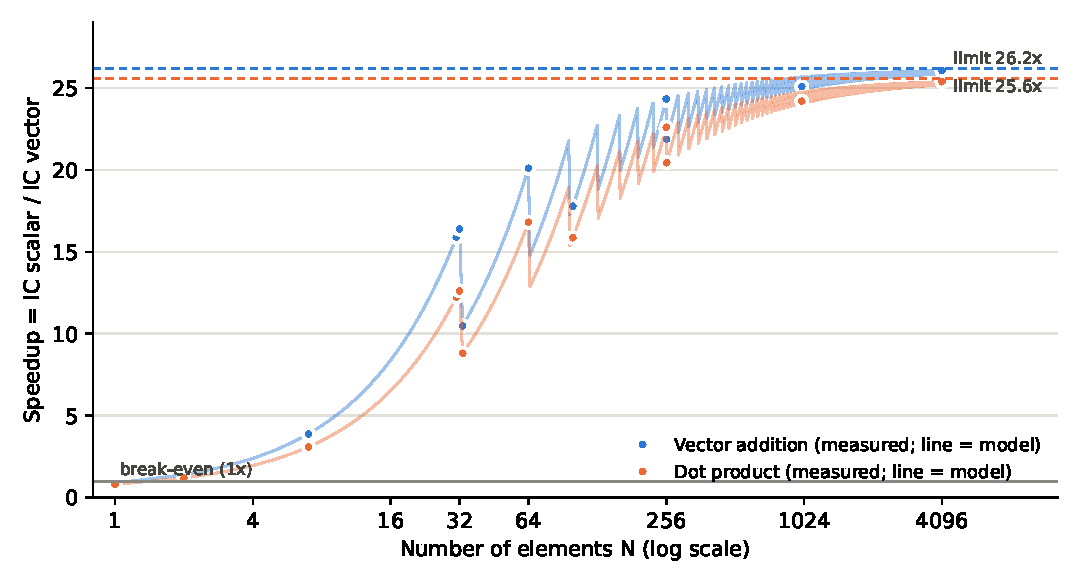
\includegraphics[width=0.92\textwidth]{speedup_vs_n.pdf}
\caption{Instruction-count speedup against array length at VLEN~=~128. Points: measured on
Kites. Lines: the model of this section. Dashed: the limits $9\cdot32/11$ and $8\cdot32/10$.}
\label{fig:speedup}
\end{figure}

\subsection{Instruction mix}

Table~\ref{tab:mix} splits the executed instructions by class, from the simulator's
statistics. In the scalar loops most instructions are \emph{loop overhead}, not arithmetic. In
the scalar addition at $N=256$, only 256 of 2{,}311 instructions (11\%) are the additions:
\begin{itemize}
  \item 768 (33\%) are loads and stores;
  \item 1{,}031 (45\%) are pointer and counter updates and set-up;
  \item 256 (11\%) are branches.
\end{itemize}
The vector version replaces all 256 additions with 8 \code{vadd.vv}. Its overhead (one
\code{vsetvli}, the pointer updates and one branch) is paid once per 32 elements.

\begin{table}[H]
\centering\footnotesize\setlength{\tabcolsep}{4.5pt}
\caption{Instruction mix (VLEN~=~128). IPE = instructions per element = IC$/N$.}
\label{tab:mix}
\begin{tabular}{llrrrrrrrr}
\toprule
Kernel & version & ALU & load/store & branch & \code{vset} & vec.\ ld/st & vec.\ compute &
total & IPE \\
\midrule
% generated by benchmarks/edge_cases.py -- do not edit
Vector addition, $N=256$ & scalar & 1{,}287 & 768 & 256 & 0 & 0 & 0 & 2{,}311 & 9.027 \\
 & vector & 47 & 0 & 8 & 8 & 24 & 8 & 95 & 0.371 \\
\midrule
Vector addition, $N=4{,}096$ & scalar & 20{,}487 & 12{,}288 & 4{,}096 & 0 & 0 & 0 & 36{,}871 & 9.002 \\
 & vector & 647 & 0 & 128 & 128 & 384 & 128 & 1{,}415 & 0.345 \\
\midrule
Dot product, $N=256$ & scalar & 1{,}288 & 513 & 256 & 0 & 0 & 0 & 2{,}057 & 8.035 \\
 & vector & 39 & 1 & 8 & 9 & 16 & 18 & 91 & 0.355 \\
\midrule
Dot product, $N=4{,}096$ & scalar & 20{,}488 & 8{,}193 & 4{,}096 & 0 & 0 & 0 & 32{,}777 & 8.002 \\
 & vector & 519 & 1 & 128 & 129 & 256 & 258 & 1{,}291 & 0.315 \\

\bottomrule
\end{tabular}
\end{table}

The instructions per element fall from about 9 (addition) and 8 (dot product) to about
0.35 and 0.32. A scalar loop can never go below one instruction per element per operation; a
vector loop shares each instruction among $vl$ elements.

\subsection{Memory traffic, branches and vector utilisation}

\begin{table}[H]
\centering\footnotesize\setlength{\tabcolsep}{4.5pt}
\caption{Memory instructions, bytes, branches and elements per vector instruction
(scalar / vector, VLEN~=~128).}
\label{tab:mem}
\begin{tabular}{lrrrrrrr}
\toprule
Kernel & $N$ & memory instr. & reduction & bytes moved & branches & elem./vec.\ instr. &
speedup \\
\midrule
% generated by benchmarks/edge_cases.py -- do not edit
Vector addition & 256 & 768 / 24 & 32.0 & 3{,}072 / 3{,}072 & 256 / 8 & 32.0 & 24.3 \\
Vector addition & 4{,}096 & 12{,}288 / 384 & 32.0 & 49{,}152 / 49{,}152 & 4{,}096 / 128 & 32.0 & 26.1 \\
Dot product & 256 & 513 / 17 & 30.2 & 2{,}052 / 2{,}052 & 256 / 8 & 30.2 & 22.6 \\
Dot product & 4{,}096 & 8{,}193 / 257 & 31.9 & 32{,}772 / 32{,}772 & 4{,}096 / 128 & 31.9 & 25.4 \\

\bottomrule
\end{tabular}
\end{table}

\begin{itemize}
  \item \textbf{Bytes moved are identical} for the two versions (for example $3 \cdot 256 \cdot
        4 = 3{,}072$ bytes for addition at $N=256$). Both versions really transfer the same
        data; the vector version simply does it with 32$\times$ fewer instructions, because one
        \code{vle32.v} with $vl=32$ moves 128 bytes where one \code{lw} moves 4.
  \item \textbf{Branches} fall from one per element ($N$) to one per pass ($P$): 256 to 8, and
        4{,}096 to 128.
  \item \textbf{Elements per vector instruction} is the average $vl$. For addition it is the
        full VLMAX of 32, so the vector registers are always full. For the dot product it is
        slightly lower (30.2 at $N=256$) because \code{vmv.s.x} and \code{vmv.x.s} work on a
        single element. Over 4{,}096 elements this matters less (31.9).
\end{itemize}

%==============================================================================================
\section{Conclusions}
%==============================================================================================

\begin{itemize}
  \item Both kernels are correct on Kites in all \runsTotal{} runs: every length from 0 (vector)
        and 1 to 4{,}096, partial last passes, 32-bit overflow, VLEN from 128 to 1{,}024 bits, and
        the single-cycle and both hazard-detecting pipelined VMs. No store ever went past the end
        of the output.
  \item The measured instruction counts equal the analytic model in every case, so the speedup
        is fully explained by the loop structure: $S \approx k_s\,\mathrm{VLMAX}/k_v$, with
        $k_s$ and $k_v$ the scalar and vector loop lengths (9 and 11 for addition, 8 and 10 for
        the dot product).
  \item At VLEN~=~128 the vector versions need 22--26$\times$ fewer instructions for arrays of a
        few hundred elements or more. With longer vector registers the same code gains more:
        128$\times$ (addition) and 98$\times$ (dot product) at $N=256$, VLEN~=~1024.
  \item Vectorisation does not pay off for a single element, breaks even at $N=2$, and is
        least effective just above a multiple of VLMAX, where the last pass is nearly empty.
  \item These figures are instruction counts. On the single-cycle simulator every instruction
        takes one step, so they are also the simulated speedup; on real hardware a vector
        instruction with large $vl$ usually takes several cycles, so the time speedup would be
        lower.
\end{itemize}

\appendix
\section{Reproducing the results}

\begin{lstlisting}[style=asm]
# build kites-cli (see README.md), then from the repository root:
python benchmarks/edge_cases.py       # all edge cases; regenerates the tables and the figure
python benchmarks/run_benchmarks.py   # the five standard benchmarks (N = 256)

# a single run, with the statistics summary:
kites-cli benchmarks/programs/dot_vector.s --stats --mem-dump 0x10000000 1
kites-cli benchmarks/programs/dot_vector.s --stats --vlen 1024
\end{lstlisting}

The raw results of every run, including the full statistics, are in
\code{benchmarks/results/edge\_cases.json}.

\end{document}
